\documentclass[a4paper,12pt,polish]{book} % nie: report!
\usepackage{url}
% \usepackage{hyperref}



% \usepackage[polish]{babel}
% \usepackage[polish]{babel}
\usepackage{babel}
\usepackage[T1,plmath]{polski} % lepiej to zamiast babel!
\selectlanguage{polish}
\usepackage[utf8]{inputenc} % w razie kłopotów spróbować: \usepackage[utf8x]{inputenc}
% \usepackage{csquotes}
\usepackage[
backend=biber,
style=numeric,
sorting=ynt
]{biblatex}

\addbibresource{refs.bib} % plik z bibliografią
\usepackage{fancyhdr} % nagłówki i stopki
\usepackage{indentfirst} % WAŻNE, MA BYĆ!
\usepackage[pdftex]{graphicx} % to do wstawiania rysunków
% \usepackage{amsfonts} % pakiety od AMS, ułatwiają składanie pewnych techniczno-matematcyznych rzeczy
% \usepackage{amsmath} % to do dodatkowych symboli, przydatne
% \usepackage{amssymb} % to też do dodatkowych symboli, też przydatne
% \usepackage{amsthm}
\usepackage{xcolor}
\usepackage[pdftex,
            left=1.1in,right=1.1in,
            top=1.1in,bottom=1.1in]{geometry} % marginesy
\usepackage{float}
\usepackage[font=small,labelfont=bf]{caption}

\usepackage[colorlinks=true]{hyperref} % odnośniki interaktywne w PDFie
\hypersetup{allcolors=black}

\usepackage{listings}
\lstset{
    basicstyle=\footnotesize\tt,
    numbers=left,
    numberstyle=\tiny,
    frame=tb,
    tabsize=4,
    columns=fixed,
    showstringspaces=false,
    showtabs=false,
    keepspaces,
    commentstyle=\color{red},
    keywordstyle=\color{blue}
}
\newfloat{lstfloat}{htbp}{lolst}[chapter]
\floatname{lstfloat}{Listing}
\def\lstfloatautorefname{Listing}
\include{colors.tex}
% jeśli potrzeb, można oczywiście wstawić inne pakiety i swoje definicje...



% definicje nagłówków i stopek
\pagestyle{fancy}
\renewcommand{\chaptermark}[1]{\markboth{#1}{}}
\renewcommand{\sectionmark}[1]{\markright{\thesection\ #1}}
\fancyhf{}
\fancyhead[LE,RO]{\footnotesize\bfseries\thepage}
\fancyhead[LO]{\footnotesize\rightmark}
\fancyhead[RE]{\footnotesize\leftmark}
\renewcommand{\headrulewidth}{0.5pt}
\renewcommand{\footrulewidth}{0pt}
\addtolength{\headheight}{1.5pt}
\fancypagestyle{plain}{\fancyhead{}\cfoot{\footnotesize\bfseries\thepage}\renewcommand{\headrulewidth}{0pt}}


% interlinia
\linespread{1.25}



\begin{document}

\begin{titlepage}
    ~

    \begin{tabular}{c@{\hspace{21mm}}|@{\hspace{5mm}}l}
        \vspace{-20mm} &                                                                    \\
        \multicolumn{2}{l}{\hspace{-12.5mm} \includegraphics[width=8cm]{LogoUMCS.jpg}}      \\
        \multicolumn{2}{@{\hspace{20mm}}l}{\vspace{-4mm}}                                   \\
        \multicolumn{2}{@{\hspace{28mm}}l}{\Large \sf UNIWERSYTET MARII
        CURIE-SKŁODOWSKIEJ}                                                                 \\
        \multicolumn{2}{@{\hspace{28mm}}l}{\vspace{-4mm}}                                   \\
        \multicolumn{2}{@{\hspace{28mm}}l}{\Large \sf W LUBLINIE}                           \\
        \multicolumn{2}{@{\hspace{28mm}}l}{\vspace{-4mm}}                                   \\
        \multicolumn{2}{@{\hspace{28mm}}l}{\Large \sf Wydział Matematyki, Fizyki i
        Informatyki}                                                                        \\
        \multicolumn{2}{@{\hspace{28mm}}l}{\vspace{21mm}}                                   \\
                       & {\sf Kierunek: \textbf{informatyka} }                              \\
        %& {\sf Specjalność: \textbf{informatyczna}} \\ % wpisujemy tylko jeśli jest!!!
                       &                                                                    \\\\\\
                       & {\sf \large \bfseries Jan Bylina}                                  \\
                       & {\sf nr albumu: 303827}                                            \\
                       &                                                                    \\\\\\
                       & \Large \sf \bfseries Projekt oraz implementacja systemu            \\
                       & \Large \sf \bfseries gromadzenia rozproszonych danych              \\
                       & \Large \sf \bfseries z wykorzystaniem technologii LoRa             \\\\[-10pt]
                       & {\large \sf Design and implementation of the distributed data  }   \\
                       & {\large \sf collection system using LoRa technology}               \\
                       &                                                                    \\
                       &                                                                    \\
                       &                                                                    \\
                       & {\sf Praca licencjacka}                                            \\
                       & \vspace{-7mm}                                                      \\
                       & {\sf napisana w Katedrze Oprogramowania Systemów Informatycznych}  \\
                       & {\sf Instytutu Informatyki UMCS}                                   \\
                       & \vspace{-7mm}                                                      \\
                       & {\sf pod kierunkiem \bfseries dra hab. Przemysława Stpiczyńskiego} \\
        \multicolumn{2}{@{\hspace{28mm}}l}{\vspace{15mm}}                                   \\
        \multicolumn{2}{@{\hspace{28mm}}l}{\textbf{\textsf{Lublin 2023}}}
    \end{tabular}
\end{titlepage}
\sloppy



\thispagestyle{empty}


\newpage{}

\thispagestyle{empty}

\newpage{}

\tableofcontents{}


\include{src/abstract.tex}


\chapter*{Wstęp} % z gwiazdką, więc bez numerka...
\addcontentsline{toc}{chapter}{Wstęp} % ...ale w spisie treści ma być
W dzisiejszych czasach ważne jest zbieranie różnorodnych informacji, z różnych, często trudno dostępnych miejsc. W~tym celu wykorzystywane są urządzenia, które zbierają informacje o~otoczeniu, a~następnie przekazują je do systemu, który następnie je przetwarza. Tego rodzaju czujniki mogą być umieszczone w~trudno dostępnych miejscach, na przykład na wysokich budynkach czy w~głębokich studniach. Nie ma tam możliwości poprowadzenia kabli, dlatego konieczne jest zastosowanie bezprzewodowych technologii komunikacyjnych. Jedną z~takich technologii jest LoRa, która pozwala na komunikację na duże odległości, przy niskim poborze mocy.

Celem niniejszej pracy jest stworzenie systemu zbierającego dane z~rozproszonych czujników z~wykorzystaniem technologii LoRa oraz ich zapisywanie w bazie danych w~celu dalszego przetworzenia.
W ramach pracy został stworzony system zbierający dane z różnych czujników, takich jak termometry~czy higrometry.
Informacje są zbierane przez autorskie punkty dostępowe LoRa, które następnie przekazują je do serwera.
Serwer przechowuje dane w bazie danych.

%TODO: fix this
W rozdziale pierwszym zostały opisane technologie, protokoły i urządzenia wykorzystane w projekcie.
W kolejnym rozdziale przedstawiono istniejące rozwiązania, zarówno przemysłowych jak i naukowych. Zostały one również porównane z rozwiązaniem zaproponowanym w ramach pracy.
W rozdziale trzecim zostały opisane założenia projektowe oraz szczegółowa implementacja systemu.
W czwartym rozdziale został opisany proces wdrożenia systemu oraz przeprowadzone testy. W ramach testów została sprawdzona wydajność systemu. Zostały również przedstawione wnioski z testów.
W piątym rozdziale zostały przedstawione wnioski z pracy oraz możliwości rozwoju systemu.


%\include{src/tutorial.tex}


\chapter{Wykorzystane narzędzia, technologie i~protokoły}
W tym rozdziale zostaną opisane narzędzia, technologie i~protokoły wykorzystane w~projekcie.
\section{Technologia LoRa}
LoRa (ang. \emph{Long Range} — daleki zasięg) to protokół komunikacji bezprzewodowej, stworzony z myślą o~urządzeniach IoT (ang. \emph{Internet of Things} — Internet rzeczy).
Przeznaczony jest do komunikacji na duże odległości i~z~niskim zużyciem energii.
Został opracowany przez Semtech w 2013 roku, stał się wtedy otwartym standardem.
LoRa wykorzystuje zastrzeżoną technologię modulacji widma rozproszonego, która umożliwia daleki zasięg, przy ograniczonym zużyciu energii.
Implementuje on warstwę fizyczną sieci~\cite{lora:about}.

Teoretyczny zasięg sieci LoRa wynosi około 15 km w terenie wiejskim i 2--5 km w terenie zurbanizowanym.
W praktyce zasięg ten jest ograniczony przez wiele czynników, takich jak:
\begin{itemize}
    \item moc nadajnika,
    \item czułość odbiornika,
    \item przeszkody fizyczne,
    \item zakłócenia,
    \item wysokość anteny.
\end{itemize}


Więcej na temat wydajności sieci można przeczytać w~artykule~\cite{bib:lora-performance}.

\section{Urządzenia wykorzystywane w~projekcie}

W tym podrozdziale zostaną opisane urządzenia wykorzystane w~projekcie, w~tym ich najważniejsze cechy.

\subsection{ESP32}
ESP32 to jednoukładowy mikrokontroler, zaprojektowany i~produkowany przez firmę Espressif Systems.
Jego najważniejsze cechy to~\cite{ESP32:datasheet}:
\begin{itemize}
    \item energooszczędny procesor RISC o częstotliwości do 240 MHz,
    \item 520 kB pamięci SRAM,
    \item WiFi 802.11 b/g/n,
    \item Bluetooth,
    \item liczne interfejsy cyfrowe i analogowe (takie jak: UART, I2C, SPI, I2S, CAN, ADC, DAC, PWM, USB 2.0).
          %       \begin{itemize}
          %           \item UART
          %           \item I2C
          %           \item SPI
          %           \item I2S
          %           \item CAN
          %           \item ADC
          %           \item DAC
          %           \item PWM
          %           \item Ethernet MAC
          %           \item USB 2.0
          %       \end{itemize}
          % \item 32 MB pamięci flash
\end{itemize}

Powstało wiele wersji tego układu, różniące się m.in. szybkością procesora, wielkością pamięci flash, ilością pinów, interfejsów cyfrowych i~analogowych, a~także możliwością pracy w trybie bezprzewodowym lub przewodowym~\cite{ESP32:socs}.
Najczęściej układ te wykorzystywane różnych projektach IoT, zarówno jako czujniki, jak i~serwery~\cite{ESP32:datasheet}.


%  PROJECTS
W projekcie ESP32 zostało wykorzystane w dwóch płytkach TTGO T3 V1.6.1.
Jedna z płytek została wykorzystana jako przekaźnik danych pomiędzy siecią LoRa a~siecią WiFi, a druga jako cześć systemu zbierania danych z wykorzystaniem LoRa.


\subsection{Raspberry Pi Pico}

Raspberry Pi Pico to płytka z mikrokontrolerem RP2040, zaprojektowana i~produkowany przez firmę Raspberry Pi Foundation.
Charakteryzuje się ona dwurdzeniowym procesorem ARM Cortex-M0+ o~częstotliwości 133 MHz, 264 kB pamięci SRAM oraz 2 MB pamięci flash.
Płytka posiada również wiele interfejsów cyfrowych i~analogowych (takich jak: UART, I2C, SPI, I2S, ADC, DAC, PWM, USB 1.1)~\cite{PICO:datasheet}.
% \begin{itemize}
%     \item UART
%     \item I2C
%     \item SPI
%     \item I2S
%     \item ADC
%     \item DAC
%     \item PWM
%     \item USB 1.1
% \end{itemize}~\cite{PICO:datasheet,PICO:doc}
Płytka ta jest często wykorzystywana przez hobbystów do różnych projektów IoT, a~także jako sterownik silników, czy kontroler robotów\cite{PICO:doc}.

%  PROJECTS
W projekcie dwie płytki zostały wykorzystane jako część systemu zbierania danych.
% \subsection{STM32}
% STM32 to rodzina 32 bitowych mikrokontrolerów produkowanych przez firmę STMicroelectronics. Bazują one na architekturze ARM Cortex-M, oferują wysoką wydajność i energooszczędność. Cztery główne rodzaje mikrokontrolerów STM32 to:
% \begin{itemize}
%     \item Rodzina płytek z~częścią kodu F(4/5) i H — overują największą wydajność
%     \item Rodzina płytek z~częścią kodu L — oferują największą energooszczędność
%     \item Rodzina płytek z~częścią kodu G/C/F(1/3) — do zastosowań ogólnych
%     \item Rodzina płytek z częścią kodu W(L/B/BA) — do zastosowań bezprzewodowych. [SRPAWDZIĆ]
% \end{itemize}\cite{STM32:overview}
% Głównym zastosowaniem STM32 są urządzenia wbudowane, w~tym urządzenia medyczne, roboty, samochody, a~także urządzenia IoT[NEED CITE]
% % -- PROJECTS
% \\
% W projekcie wykorzystano dwie płytki STM32WL55, które zostały wykorzystane jako część systemu zbierania danych.


% \section{Języki programowania i technologie}
% \subsection{\texttt{C++} for Arduio}
% ---
\section{MicroPython for Raspberry Pi Pico}
MicroPython to lekka~i wydajna implementacja języka Python 3, która została zaprojektowana~z myślą~o urządzeniach wbudowanych.
Zawiera on okrojoną wersję biblioteki standardowej Pythona.
MicroPython jest dostępny na wiele platform,~w tym na Raspberry Pi Pico~\cite{PICO:micropython}.

\section{Protokoły komunikacyjne: MQTT}

MQTT (ang. \emph{MQ Telemetry Transport}) to lekki protokół przesyłania wiadomości, często wykorzystywany w IoT, gdzie ważna jest energooszczędność.
Oparty jest o model \emph{publish/subscribe}.
Oznacza to zorganizowanie wiadomości w tematy, a klienci mogą subskrybować określone przez siebie tematy, aby otrzymywać odpowiednie wiadomości.
Zapewnia to wydają komunikację przy małym obciążeniu systemu~\cite{protocol:mqtt}.

\section{Bazy danych i pozostałe technologie}
\subsection{InfluxDB 2}
InfluxDB 2 to baza danych szeregów czasowych, stworzona przez InfluxData, Została napisana w języku Go.
Wykorzystywana jest do zbierania danych z~, między innymi, urządzeń IoT, metryk aplikacji, monitoringu infrastruktury IT~\cite{tool:influxdb}.

\subsection{Docker}
Docker to narzędzie do wirtualizacji na poziomie systemu operacyjnego.
Pozwala ono na uruchamianie aplikacji w~kontenerach, które są odizolowane od siebie i~od systemu operacyjnego.
Kontenery mniej obciążają pamięć i procesor od wirtualnych maszyn, ponieważ nie muszą zawierać systemu operacyjnego, a~tylko potrzebne do działania aplikacji biblioteki i~pliki~\cite{tool:docker}.

\subsection{PlatformIO}
PlatformIO to narzędzie do tworzenia i~zarządzania projektami z~wykorzystaniem mikrokontrolerów.
Pozwala ono na tworzenie projektów w~językach C i~C++.
PlatformIO oferuje również możliwość zarządzania zależnościami projektu, zarządzania bibliotekami, a~także kompilację i~wgrywanie projektu na płytkę.
Najważniejszą cechą jest możliwość tworzenia projektów dla wielu platform i z wykorzystaniem równych narzędzi, w~tym dla ESP32 i~Raspberry Pi Pico, będąc jednocześnie niezależnym od jednego producenta~\cite{tool:pio}.

\begin{figure}[b!]
    \begin{center}
        \includegraphics[angle=90, width=10cm]{pic/pio.jpg}
    \end{center}
    \caption{Interfejs narzędzia PlatformIO w edytorze Visual Studio Code}\label{fig:pio}
\end{figure}



\chapter{Istniejące rozwiązania}
---
\section{LoRaWAN}
---
\subsection{The Things Network ?}
---
\subsection{ChirpStack ?}
---
\subsection{Loriot ?}
---
\section{Artykuły}
---
\section{Wpisy w sieci i blogach}


\chapter{Założenie i Implementacja}
W poniższym rozdziale zaprocentowano założenia, potrzeby~i projekt projektu Sieci Meash na bazie LoRa

\section{Podstawowe cele sieci}
System ma kilka podstawowych założeń:
\begin{itemize}
    \item Jeden centralny punkt gromadzenia danych
    \item Zapisywanie danych do bazy danych szeregów czasowych, w celu ich dalszego przetwarzania
    \item Zbieranie danych z dużego obszaru
    \item Niezależność od istniejących metod przesyłu danych (WiFI, Sieci komórkowe, Łączność satelitarna)
    \item Niezależność od platformy sprzętowej
    \item Zapewniać możliwie dużą dostarczalność pakietów
    \item Dane czasowe nie muszą być super dokładne (dopuszczalne są drobne opóźnienia)
    \item Węzły sieci tylko wysyłają dane, same nie konsumują przychodzących wiadomości
\end{itemize}

\section{Części sieci}
W celu uzyskania wyżej wspomnianych założeń, zaproponowano system złożonych z kilku części:
\subsection{Węzły sieci}
Węzły sieci to urządzenia wyposażone w moduł LoRa i odpowiednie oprogramowanie pozwalające na pełną obsługę sieci. Gdy węzeł odbierze wiadomość, sprawdza jej poprawność i rozsyła ja dalej w celu zapewnienia jak największego zasięgu i wystarczalności

Urządzenie to może być również wyposażone w różnego rodzaju czujniki, które dostarczają danych bazy danych.

\subsection{Stacja przekaźnikowa}
Stacja przekaźnikowa to urządzenie wyposażone zarówno w moduł LoRa jak i moduł umożliwiający komunikację z siecią Internet (np. moduł WiFI lub moduł bazy Ethernet).

Urządzenie to odbiera przychodzące wiadomości LoRa i przesyła je do brokera wiadomości

\subsection{Broker wiadomości}
Broker wiadomości to program, działający na komputerze mającym dostęp do sieci, umożliwia on wydajną komunikację pomiędzy Stacją Przekaźnikową a Bazą Danych

\subsection{Baza danych}
Baza Danych umożliwiająca zapisywanie sporej ilości danych, uwzględniając również ich czas (baza danych szeregów czasowych).
O zapisy danych z brokera wiadomości do bazy danych dba osobny program, który powinien sprawdzać również poprawność tych wiadomości, jak i dbać o to by nie zapisywać powtórzonych wiadomości

\section{Wiadomości}
Każda z wiadomości przesyłanych za pomocą tych sieci powinna mieć formę jak zaprezentowano na listingu~\ref{lst:packet_format}

Zawiera ona pola:
\begin{itemize}
    \item \texttt{ttl} — [Ang. time to live — czas życia] Wartość określająca maksymalną liczbę skoków pomiędzy węzłami sieci. Domyślnie wynosi 10, może zostać wydłużona w zależności od wielkości planowanej sieci
    \item \texttt{m\_id} — UUID \cite{RFC:uuid} wiadomości, gwarantujący niepowtarzalności tej wiadomości. Ułatwia również jej dalsze przetwarzanie
    \item \texttt{d\_id} — numer identyfikacyjny urządzenia z którego pochodzi wiadomość
    \item \texttt{values} — słownik zawierający dane z urządzenia, do zapisania w bazie
\end{itemize}

\begin{lstfloat}[b]
    \lstset{language=JavaScript}
    \begin{lstlisting}[frame=single]
{
    "d_id": "id_233",
    "values": {
        "temp": "21",
        "hum": "50",
        "press": "1000",
        "light": "100",
        "co2": "1000",
        "pm25": "10",
        "pm10": "20"
    },
    "ttl": 10,
    "m_id": "eaa17a7b-9388-43b6-9310-731c942fc6b9"
}          
\end{lstlisting}
    \caption{Przykładowa wiadomość przesyłana przez system}\label{lst:packet_format}
\end{lstfloat}

\section{Obsługa protokołu}

\subsection{Działanie węzłów}
Wiadomości generowane są przez węzły sieci, zawierając wszystkie niezbędne pola (wymienione wyżej) i odczyty z czujników zamieszczonych na węźle. Następnie zostaje ona rozesłana do wszystkich węzłów w zasięgu (broadcasting).

Węzeł odbierając wiadomość, sprawdza jej poprawność (czy jest odpowiednio sformatowana, czy zawiera wszystkie potrzebne pola), i jeżeli wiadomość jest poprawna,a pole \texttt{ttl} jest większe od 0 rozsyła wiadomość dalej.
Sprawdzanie wiadomości odbywa się by wyeliminować wiadomości niepoprawne z sieci.

% TODO wstawić rysunek 

\subsection{Działanie przekaźnika}
Przekaźnik odbiera wiadomości, i przesyła je do brokera wiadomości. Nie sprawdza poprawności wiadomości by zapewnić maksymalną wydajność i niezawodność.

\subsection{Działanie bazy danych i programu zapisującego dane}
Program pobiera kolejne wiadomości od brokera i przetwarza je w kolejności:
\begin{enumerate}
    \item Sprawdzenie poprawności wiadomości
    \item \label{itm:powtorki} Sprawdzenie czy wiadomość nie została już sprawdzona (na podstawie pola \texttt{m\_id})
    \item Zapisanie danych ze słownika \texttt{values} do bazy danych i przyporządkowanie ich do \texttt{d\_id}
    \item Zapisanie w pamięci operacyjnej \texttt{m\_id}, potem do wykorzystania w~kroku \ref{itm:powtorki}
\end{enumerate}

\section{Implementacja}
\subsection{Implementacja przykładowych węzłów sieci}
W wyniku pracy nad systemem zbierania danych przygotowano implementację węzłów sieci w wykonrzystaniem 3 platform sprzętowych:
% TODO sprawdzić jakie dokładnie to modele
\begin{itemize}
    \item Rasberry Pi Pico +
    \item ESP32 TTYGO
    \item STM32 WL\dots
\end{itemize}


\chapter{Wdrożenie i testy}
W tym rozdziale zostanie opisane wdrożenie systemu oraz przeprowadzone testy.
\section{Wdrożenie}
System został wdrożony 1~maja 2023 roku.
Wdrożenie polegało na uruchomieniu serwera z~bazą danych, jednej stacji przekaźnikowej oraz uruchomieniu trzech urządzeń pomiarowych.

\subsubsection{Węzły sieci}
% Węzły sieci zostały umieszczone w trzech różnych miejscach w Lublinie. Pierwszy z nich został umieszczony na dachu budynku Wydziału Matematyki, Fizyki i Informatyki UMCS. Drugi został umieszczony na dachu budynku Wydziału Elektrotechniki i Informatyki Politechniki Lubelskiej. Trzeci został umieszczony na dachu budynku Wydziału Informatyki Politechniki Lubelskiej. Wszystkie urządzenia zostały umieszczone na wysokości 20 metrów nad poziomem gruntu. Wszystkie urządzenia zostały umieszczone na zewnątrz, w~specjalnych obudowach, które zapewniają ochronę przed warunkami atmosferycznymi. Wszystkie urządzenia zostały zasilone z sieci elektrycznej.

Trzy węzły sieci zostały rozmieszczone na małym obszarze, około 30 metrów od siebie, w~dwóch budynkach.
Dwa urządzenia (jedno Raspberry Pi Pico i~jedno TTGO LoRa32) zasilane są z~sieci, jedno za pomocą baterii (Raspberry Pi Pico).
Urządzenia zostały połączone z~czujnikami za pomocą zwykłych kabli prototypowych, jak na rysunku~\ref{rys:wezel1}. %i~\ref{rys:wezel2}.
Przykład urządzenia wykorzystującego wbudowane czujniki został zaprezentowany na rysunku~\ref{rys:wezel2}.

\begin{figure}[b!]
    \begin{center}
        % 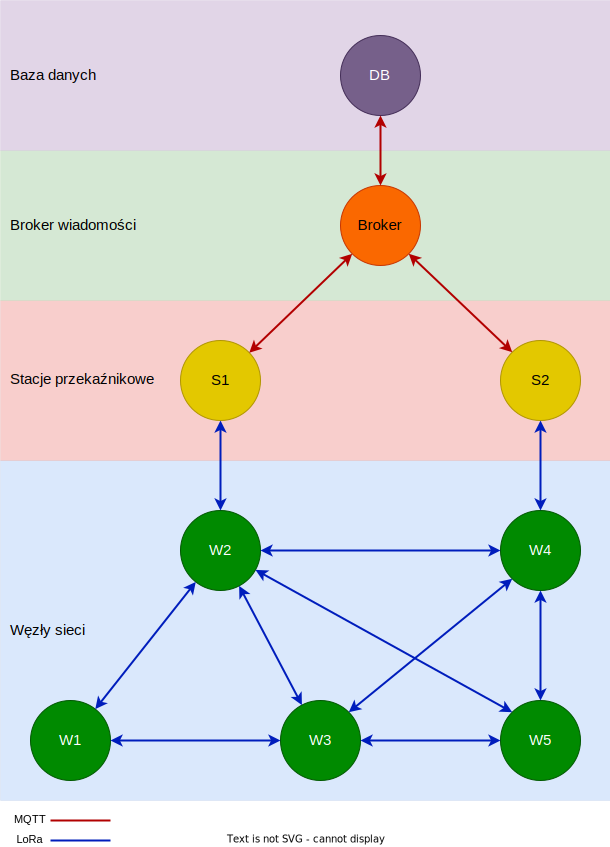
\includegraphics[width=3cm]{pic/diagram-systemu.png}
        \includegraphics[width=13cm]{pic/wezel1.jpg}
    \end{center}
    \caption{Zdjęcie węzła sieci opartego o~Raspberry Pi Pico wraz z baterią}\label{rys:wezel1}
\end{figure}

\begin{figure}[b!]
    \begin{center}
        \includegraphics[width=13cm]{pic/logi-pico.png}
        % \includegraphics[height=13cm]{pic/logi-pico.png}
    \end{center}
    \caption{Zrzut ekranu zawierający logi z~jedno z węzłów sieci(Raspberry Pi Pico)}\label{rys:logi-pico}
\end{figure}

\begin{figure}[b!]
    \begin{center}
        \includegraphics[width=13cm]{pic/wezel2.jpg}
    \end{center}
    \caption{Zdjęcie węzła sieci opartego TTGO T3 LoRa32}\label{rys:wezel2}
\end{figure}

\subsubsection{Stacja przekaźnikowa}
Stacja przekaźnikowa została umieszczona w~pobliżu głównego serwera, w~zasięgu sieci WiFi, wewnątrz budynku.
Urządzenie zostało zasilone z~sieci elektrycznej.
Na ekranie urządzenia wyświetlane są informacje o~stanie urządzenia, jak na rysunku~\ref{rys:stacja1}.

\begin{figure}[b!]
    \begin{center}
        \includegraphics[width=13cm]{pic/stacja1.jpg}
    \end{center}
    \caption{Zdjęcie stacji przekaźnikowej opartej o~TTGO T3 LoRa32}\label{rys:stacja1}
\end{figure}


\subsubsection{Serwer testowy}
Na serwerze testowym zostały uruchomione wszystkie usługi, które zostały wykorzystane w projekcie, w~szczególności:
\begin{itemize}
    \item Mosquitto (patrz str.~\pageref{impl:mosquitto})
    \item InfluxDB 2 (patrz str.~\pageref{impl:db})
    \item Program zapisujący do InfluxDB 2 (patrz str.~\pageref{impl:save})
    \item Redis (patrz str.~\pageref{impl:redis})
\end{itemize}
Serwer został uruchomiony na maszynie wewnątrz budynku, w~sieci lokalnej.
Na serwerze został uruchomiony system operacyjny Debian 11.
Maszyna została wyposażona w~procesor Intel Core i5-480M, 2 GB pamięci RAM oraz dysk SSD o pojemności 256 GB.
Wszystkie usługi zostały uruchomione w~kontenerach Dockera~\cite{tool:docker}, w jednej sieci wirtualnej, w~celu zapewnienia komunikacji między nimi.

\subsubsection{Broker wiadomości}
Broker wiadomości został uruchomiony na wspólnym serwerze wewnątrz budynku.
Broker został zabezpieczony hasłem, które zostało zapisane w~pliku konfiguracyjnym.
Wszystkie urządzenia zostały skonfigurowane tak, aby połączyć się z~brokerem za pomocą tego hasła.
Nie zostało użyte szyfrowanie TLS, ponieważ sieć wewnętrzna została uznana za bezpieczną, a użycie szyfrowania zwiększyło by skomplikowanie systemu.

\subsubsection{Baza danych i program zapisujący dane}
Baza danych wraz z programem zapisującym dane zostały uruchomione na wspólnym serwerze wewnątrz budynku.
Baza danych została zabezpieczona tokenem dostępu, który został zapisany w~pliku konfiguracyjnym.
Program zapisujący dane został skonfigurowany tak, aby połączyć się z~bazą danych za pomocą tego tokenu.
% Nie zostało użyte szyfrowanie TLS.
Zarówno baza danych, jak i program zapisujący dane zostały uruchomione w kontenerach Dockera, w celu zapewnienia izolacji i~łatwości konfiguracji.
Na rysunku~\ref{rys:influxdb-web} został przedstawiony zrzut ekranu interfejsu użytkownika InfluxDB 2.
Na rysunku~\ref{rys:logi-connector} został przedstawiony zrzut ekranu zawierający logi programu zapisującego pomiary do bazy InfluxDB~2.

\begin{figure}[b!]
    \begin{center}
        \includegraphics[width=13cm]{pic/influxdb-web.png}
    \end{center}
    \caption{Zrzut ekranu interfejsu użytkownika InfluxDB 2}\label{rys:influxdb-web}
\end{figure}

\begin{figure}[b!]
    \begin{center}
        \includegraphics[width=13cm]{pic/logi-connector.png}
    \end{center}
    \caption{Zrzut ekranu zawierający logi programu zapisującego pomiary do bazy InfluxDB 2}\label{rys:logi-connector}
\end{figure}

\subsubsection{Redis}
Redis został uruchomiony na wspólnym serwerze wewnątrz budynku.
Redis pozostał niezabezpieczony, ponieważ został udostępniony w~sieci wewnętrznej.
Tutaj również nie zostało użyte szyfrowanie.
Redis został uruchomiony w kontenerze Dockera, w celu zapewnienia izolacji i~łatwości konfiguracji.

% picure of server
\section{Testy}
System został przetestowany pod kątem poprawności działania, wydajności oraz niezawodności.
Testy zostały przeprowadzone w~dniach od 1 do 14 maja 2023 roku.

\subsection{Poprawność działania}
Poprawność działania była weryfikowań na kilka, następujących sposobów:

\subsubsection{Weryfikacja poprawności działania urządzeń pomiarowych}

Weryfikacja poprawności działania urządzeń pomiarowych została przeprowadzona dla odczytów temperatury.
Test ten polegał na porównaniu odczytów z~dwóch różnych czujników temperatury w tym sam czasie.
Porównania dokonano pomiędzy czujnikiem DHT11 a~czujnikiem DS18B20.
Odczyty zostały zapisane do pliku CSV a~następnie porównane.
Przykładowe wyniki testów zostały przedstawione na rysunku~\ref{rys:dht-vs-ds}.

\begin{figure}[b!]
    \begin{center}
        \includegraphics[width=15cm]{pic/dht-vs-ds.png}
    \end{center}
    \caption{Wykres temperatury od czasu dla czujników \texttt{DHT11} i~\texttt{DS18B20}}\label{rys:dht-vs-ds}
\end{figure}

Jak widać na załączonym rysunku, wyniki odczytów są bardzo zbliżone (maksymalna różnica pomiarów to 1°C), co świadczy o~poprawności działania urządzeń pomiarowych.

\subsubsection{Weryfikacja poprawności działania całego sytemu}
Weryfikacja poprawności działania całego systemu została przeprowadzona poprzez porównywanie pakietów wysyłanych przez urządzenia pomiarowe z~pakietami zapisanymi w~bazie danych.
Próba ta polegała na porównaniu wszystkich pól pakietów.
Porównanie to odbywało się ręcznie i~dotyczyło tylko kilku pakietów.
Dodatkowo weryfikowano poprawność działania poprzez sprawdzenie zmian we wskazaniach czujników.
Przejścia dla temperatury i~wilgotności były bardzo płynne, co świadczy o~poprawności działania systemu.
Przejścia dla liczb losowych były bardzo chaotyczne, co również świadczy o~poprawności działania systemu.
Przykładowe wyniki testów zostały przedstawione na rysunku~\ref{rys:porownanie-hum}.
% TODO: WIęcej wyników testów ?
\begin{figure}[b!]
    \begin{center}
        \includegraphics[width=15cm]{pic/diagram-humidity.png}
    \end{center}
    \caption{Wykres wilgotności od czasu(w okresie od 2 Maja 2023 do 7 Maja 2023)}\label{rys:porownanie-hum}
\end{figure}


Dzięki wyżej wymienionym testom, udało się stwierdzić, że system działa poprawnie.

\subsection{Wydajność}
Testy wydajności zostały przeprowadzone w~celu sprawdzenia, czy system jest w~stanie obsłużyć wszystkie pakiety wysyłane przez urządzenia pomiarowe.
Testy zostały przeprowadzone w dwóch etapach:
\begin{itemize}
    \item testy wydajności stacji przekaźnikowej,
    \item testy wydajności węzłów sieci.
\end{itemize}

\subsubsection{Testy wydajności stacji przekaźnikowej}
Testy zostały przeprowadzone w następujący sposób: z~trzech węzłów sieci były emitowane pakiety w bardzo krótkich odstępach czasu (co 10 sekund).
Wszystkie pakiety były wysyłane do stacji przekaźnikowej.
Następnie przekazywała ona te pakiety do brokera wiadomości.
Wszystkie pakiety były zapisywane w~bazie danych.

W~wyniku testów zostało stwierdzone, że stacja przekaźnikowa jest w stanie obsłużyć wszystkie pakiety wysyłane przez węzły sieci poprawnie.

\subsubsection{Testy wydajności węzłów sieci}
Testy zostały przeprowadzone w~następujący sposób: z~trzech węzłów sieci były emitowane pakiety w~bardzo krótkich odstępach czasu (co 10 sekund).
Weryfikacji podlegało to, czy wszystkie pakiety zostały wysłane ponownie rozgłoszone przez węzły sieci.
Wszystkie pakiety były odbierane również przez stację przekaźnikową.

W wyniku testów zostało stwierdzone, że węzły sieci są w stanie obsłużyć wszystkie pakiety wysyłane przez sieci poprawnie.
Przykładowe wyniki testów zostały przedstawione na rysunku~\ref{rys:odbijanie-pakietu}.

\begin{figure}[b!]
    \begin{center}
        \includegraphics[width=13cm]{pic/odbijanie-pakietu.png}
    \end{center}
    \caption{Przykładowy pakiet, odebrany przez jeden z~węzłów sieci}\label{rys:odbijanie-pakietu}
\end{figure}

\section{Zauważone problemy}
W~trakcie testów zostały zauważone następujące problemy:
\subsubsection{Błędne pakiety}
\begin{itemize}
    \item Węzły sieci czasami odbierały błędne pakiety, jak na rysunku~\ref{rys:zly-pakiet}. Problem ten został rozwiązany prze sprawdzanie czy odebrany pakiet jest poprawny, a~w~przypadku błędu, pakiet był odrzucany.
    \item Przekaźnik sieci czasami przekazuje błędne pakiety do brokera (jak na rysunku~\ref{rys:zly-pakiet}). Problem ten został rozwiązany przez sprawdzanie czy odebrany pakiet jest poprawny na poziomie programu zapisującego do bazy danych, a~w~przypadku błędu, pakiet jest odrzucany. Można byłoby sprawdzać poprawność pakietu na poziomie przekaźnika, ale obniżyłoby to wydajność systemu.
\end{itemize}

\begin{figure}[b!]
    \begin{center}
        \includegraphics[width=13cm]{pic/zly-pakiet.png}
    \end{center}
    \caption{Przykładowy błędny pakiet odebrany przez jeden z~węzłów sieci}\label{rys:zly-pakiet}
\end{figure}

\subsubsection{Błędy pochodzenia zewnętrzego}
Jak łatwo zauważyć na wykresie~\ref{rys:diagram-scat}, niestety w~bazie danych pojawiają się luki w~zapisanych danych.
Takie luki spowodowane są brakami zasilania spowodowane przez osoby obsługujące ten system w~czasie testów.
Niektóre czujniki traciły zasilanie przez nieuważne zmiany kabli zasilających czy wyczerpanie się baterii.
Jednym z~możliwych rozwiązań jest baterii o większej pojemności w~każdym węźle sieci.

\begin{figure}[b!]
    \begin{center}
        \includegraphics[width=13cm]{pic/diagram-scat-humm.png}
    \end{center}
    \caption{Szczegółowych diagram danych zapisanych w~bazie między 4 Maja, a 6 Maja 2023}\label{rys:diagram-scat}
\end{figure}

%  TODO: add more screenshots


\chapter{Perspektywy rozwoju i dalsze badania}

\section{Rozwój projektu}
W~trakcie pracy nad projektem udało się zrealizować wszystkie założenia projektowe.
Wszystkie urządzenia zostały zaprogramowane i~skonfigurowane, a~system zbierania danych został zaimplementowany.
Wszystkie urządzenia zostały przetestowane i~działają poprawnie.
Jednak w~przyszłości można rozwinąć projekt o~kilka funkcjonalności i~usprawnień, które mogą zwiększyć użyteczność systemu.

\subsection{Optymalizacja energetyczna węzłów sieci}
\subsubsection*{Zmniejszenie częstotliwości wysyłania pakietów}
Implementacja węzłów sieci w~obecnej wersji skupia się na stabilności i~poprawności działania.
Jednak w~przyszłości można rozwinąć projekt o~funkcjonalność optymalizacji energetycznej węzłów sieci.
W~obecnej wersji węzły sieci wysyłają pakiety w~stałych odstępach czasu.
Jednak w~przypadku, gdy węzły sieci nie wykryją żadnych zmian w~otoczeniu, nie ma potrzeby wysyłania pakietów.
W~takiej sytuacji można zastosować algorytm, który będzie sprawdzał, czy w~otoczeniu węzła sieci występują jakieś zmiany.
Jeśli nie, to węzeł sieci będzie wysyłał pakiety w~dłuższych odstępach czasu.
Dzięki temu można zaoszczędzić energię węzłów sieci.

\subsubsection{Usypianie węzłów sieci}

Wiele mikrokontrolerów posiada funkcjonalność głębokiego uśpienia.
W~takim trybie mikrokontroler zużywa bardzo mało energii.
Jednak w~takim trybie mikrokontroler nie jest w~stanie wykonywać żadnych operacji.
Należałoby rozpoznać czy tryby uśpienia zaproponowanych przez producentów mikrokontrolerów są wystarczające do zastosowania w~projekcie.
Jeśli tak, to można zastosować tryby uśpienia w~węzłach sieci, które nie będą wysyłały pakietów przez dłuższy czas.

\subsubsection*{Większa bateria}
W celu wydłużenia czasu działania węzłów sieci można również zastosować większe baterie. Wydłużyłoby to nieprzerwany czas pracy na baterii.

\subsubsection*{Zastosowanie innych technologii}
W~celu optymalizacji energetycznej węzłów sieci można również zastosować inne technologie do oprogramowania węzłów sieci.
W~obecnej wersji węzły sieci niektóre węzły sieci zostały zaprogramowane w~języku MicroPython, a~inne w~języku C++.
W~przyszłości można przepisać wszystkie węzły sieci na jeden język programowania.
W~takim przypadku można zastosować język C++, który jest bardziej wydajny od języka MicroPython.
Dzięki temu można zwiększyć wydajność węzłów sieci przy jednoczesnej zwiększonej wydajności energetycznej.
% TODO: dodać bibliografi o wydjaności języków programowania

\subsection{Bezpieczeństwo}

\subsubsection{Autoryzacja węzłów sieci}
W~obecnej wersji systemu węzły sieci nie są autoryzowane.
W~takiej sytuacji każdy węzeł sieci może dołączyć do sieci i~wysyłać pakiety.
Jednak w~przyszłości można rozwinąć projekt o~funkcjonalność autoryzacji węzłów sieci.
Węzły sieci będą musiały autoryzować się przed dołączeniem do sieci.
Dzięki temu można zwiększyć wtedy bezpieczeństwo systemu.

\subsubsection{Szyfrowanie wiadomości}
W~obecnej wersji systemu wiadomości wysyłane przez węzły sieci nie są szyfrowane.
Biorąc pod uwagę specyfikę protokołu LoRa wiadomości są rozgłaszane w formie broadcastu, więc mogą zostać odebrane przez dowolne urządzenie.
W~przyszłości można rozwinąć projekt o~funkcjonalność szyfrowania wiadomości.
W~takiej sytuacji węzły sieci będą szyfrowały wiadomości przed wysłaniem ich do stacji przekaźnikowej.
Następnie stacja przekaźnikowa będzie odszyfrowywała wiadomości przed przekazaniem ich do brokera wiadomości.
Dzięki temu można zwiększyć bezpieczeństwo systemu.

Należałoby rozpoznać, czy szyfrowanie wiadomości nie spowoduje zbyt dużego spadku wydajności systemu.
W~takim przypadku można zastosować szyfrowanie wiadomości tylko w~sytuacji, gdy w~wiadomości znajdują się dane poufne.

Należałoby również sprawdzić, jaka forma szyfrowania jest najbardziej odpowiednia do zastosowania w~projekcie.
W~tym celu można przeprowadzić badania porównujące różne formy i~algorytmy szyfrowania pod względem wydajności i~bezpieczeństwa.

Jeżeli zdecydowano by się na implementacje szyfrowania z~wykorzystaniem klucza, to należałoby rozpoznać, jak klucz będzie przekazywany do węzłów sieci.
W~tym celu można zastosować algorytm wymiany klucza Diffiego-Hellmana.
Dzięki temu klucz szyfrowania będzie przekazywany bezpiecznie.

W celu szyfrowania wiadomości należałoby również rozpoznać, jakie algorytmy szyfrowania są dostępne w~mikrokontrolerach.
W~tym celu można przeprowadzić badania porównujące różne mikrokontrolery pod względem dostępnych algorytmów szyfrowania.

\subsection{Komunikacja dwukierunkowa}
W~obecnej wersji systemu komunikacja między węzłami sieci a~stacją przekaźnikową jest jednokierunkowa.
W~przyszłości można rozwinąć projekt o~funkcjonalność komunikacji dwukierunkowej.
W~takiej sytuacji węzły sieci będą mogły odbierać wiadomości od stacji przekaźnikowej.
Dzięki temu można zwiększyć użyteczność systemu, chociażby poprzez możliwość zdalnego sterowania węzłami sieci.
% TODO:  co to arduino
\subsection{Przygotowanie nowych węzłów sieci}
W~obecnej wersji systemu została przygotowana implementacja węzłów sieci, która jest kompatybilna z~platformami opartymi o Arduino lub MicroPython.
Podczas prac nad następną iteracją projekt można rozwinąć o~funkcjonalność przygotowania nowych węzłów sieci.
W~takiej sytuacji można przygotować implementację węzłów sieci, która będzie kompatybilna z~innymi platformami (takimi jak STM32).
Dzięki temu można zwiększyć uniwersalność systemu.

\section{Dalsze badania}

\subsection{Badania wydajnościowe dużej sieci}
W~trakcie pracy nad projektem zostały przeprowadzone testy wydajnościowe bardzo małej sieci (trzy węzły).
Powinny jednak zostać przeprowadzone badania wydajnościowe dużej sieci.
W~takiej sytuacji można przetestować wydajność systemu w~sytuacji, gdy w~sieci znajduje się dużo węzłów sieci na znacznej powierzchni.
Dzięki temu można sprawdzić, czy system jest w~stanie obsłużyć dużą liczbę węzłów.

\subsection{Badania zużycia energii}
W~trakcie przyszłych prac nad projektem należałoby przeprowadzić badania konsumpcji energii węzłów sieci.
W~takiej sytuacji można sprawdzić, jak długo węzły sieci mogą działać na baterii.
Należałoby również zoptymalizować zużycie energii węzłów sieci.
Dzięki temu można zwiększyć czas działania węzłów sieci na zasilaniu bateryjnym.

\subsection{Badania zasięgu sieci}
W~trakcie przyszłych prac nad projektem należałoby przeprowadzić badania zasięgu sieci.
W~takiej sytuacji można sprawdzić, jak daleko od siebie mogą znajdować się węzły sieci.
Dzięki temu można sprawdzić, jakie są ograniczenia zasięgu sieci.


\chapter*{Podsumowanie}

\addcontentsline{toc}{chapter}{Podsumowanie}



\listof{lstfloat}{Spis listingów} % jeśli są listingi
\addcontentsline{toc}{chapter}{Spis listingów}

\listoftables{} % jeśli są tabele
\addcontentsline{toc}{chapter}{Spis tabel}

\listoffigures{} % jeśli są rysunki
\addcontentsline{toc}{chapter}{Spis rysunków}


\addcontentsline{toc}{chapter}{Bibliografia} % też ręczne dodanie do spisu treści, jak Wstęp

\printbibliography % wydruk bibliografii
% \bibliographystyle{plain}
% \begin{thebibliography}{99}
%     \bibitem{bib:a} aaaaaaaa
%     \bibitem{bib:b} bbbbbbbb
%     \bibitem{bib:esp32-all-socs} \href{https://www.espressif.com/en/products/socs}(dostęp: 15.04.2023)
% \end{thebibliography}




\end{document}
